\subsection{Simple Polygons}
\label{sec:warm-up}

To get a sense of the types of problems we will encounter,
we begin by deriving a formula for the area
of a simple polygon on the sphere in terms of the 
interior angles.
\begin{theorem}\label{thm:triangle}
In the plane, the sum of the interior angles of a triangle is $\pi$.
\end{theorem}
\begin{proof}
Draw a line parallel to one edge through the opposite vertex.
By alternating interior angles in the plane, the sum of the angles
in the triangle equal  a straight line.
See \figref{angles} for an illustration. 



\begin{figure}[htb]
\centering
\includegraphics[width=.3\textwidth]{background/interior-angles-triangle}
\caption{A proof that, in the plane, the sum of the angles of a triangle is $\pi$.}
\label{fig:angles}
\end{figure}

\end{proof}



Consider any simple polygon in the plane $P$ with $n$ vertices. 
Then $P$ can be triangulated with $n-2$ triangles \cite{orourke_computational_1994}.
Thus, when we traverse $P$ we go around $n-2$ triangles each contributing
$\pi$.
We have
\begin{corollary}\label{cor:angles}
In the plane, any simple polygon $P$ with $n$ vertices,
the sum of the interior angles of $P$ is $(n-2)\pi$.

\end{corollary}

Now consider a triangle on the two dimensional sphere as in \figref{sphere-triangle}.

\begin{figure}[htb]
\centering
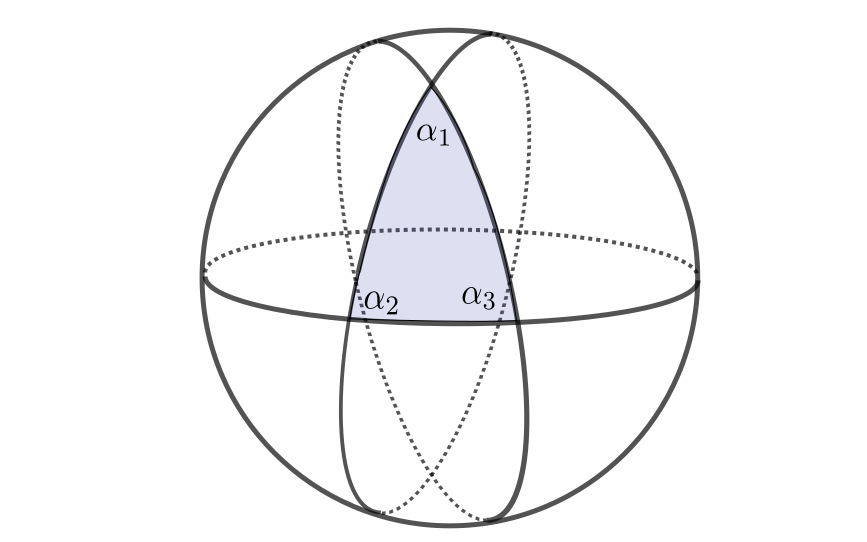
\includegraphics[width=.5\textwidth]{background/sphere-triangle}
\caption{A triangle on the sphere.}
\label{fig:sphere-triangle}
\end{figure}
A spherical \EMPH{lune} is the region on a sphere bounded by two half great circles
with angle $\alpha$ the area of a lune is denoted $A(\alpha)$,
 see \figref{lune}.
On the unit sphere, the area of a lune is proportional to $\alpha$. 
If $\alpha=0$ the area is zero and if $\alpha=\pi$ the area is $4\pi$.
We can add the area of two lunes in terms of their angles, 
$A(\alpha_1+\alpha_2)=A(\alpha_1)+A(\alpha_2)$ so $A$ is linear
and  $A(\alpha)=4\alpha.$


\begin{figure}[htb]
\centering
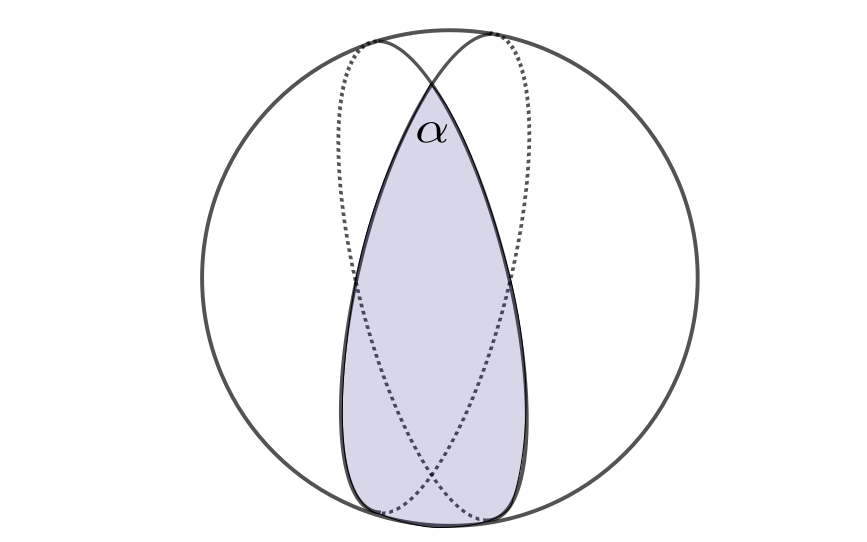
\includegraphics[width=.5\textwidth]{background/lune}
\caption{A lune with angle $\alpha$.}
\label{fig:lune}
\end{figure}

The area of a triangle on the sphere is related to the angles.

\begin{lemma}[Area of Spherical Triangle]\label{lem:spherical-triangle}
On the unit sphere, the area of a triangle with interior angles $\alpha_1, \alpha_2, \alpha_3$
is $A=\alpha_1+\alpha_2+\alpha_3-\pi$.
\end{lemma}

\begin{proof}
Any two edges of the the triangle form a lune. The collection of 
all three lunes covers the entire sphere with triangle and the antipodal triangle
are covered three times. The surface area of the unit sphere is $4\pi$.

Thus, $4\pi=2(2\alpha_1+2\alpha_2+2\alpha_3)-6A+2A$
and $A=\alpha_1+\alpha_2+\alpha_3-\pi$.
\end{proof}

As in the plane, any polygon on the sphere with $n$ vertices can be decomposed
into $n-2$ triangles. This gives a formula for the area of a simple polygon
on the sphere with interior angles $\beta_1,\beta_2,\ldots, \beta_n$.

\begin{equation} \label{eqn:sphere-area}
A=(2-n)\pi +\sum_{i=1}^n \beta_i.
\end{equation}

\eqnref{sphere-area} will be used to compute
the discrete curvature of vertex.

